\subsection{Memory Execution Pipeline}

\begin{figure}
    \centering
    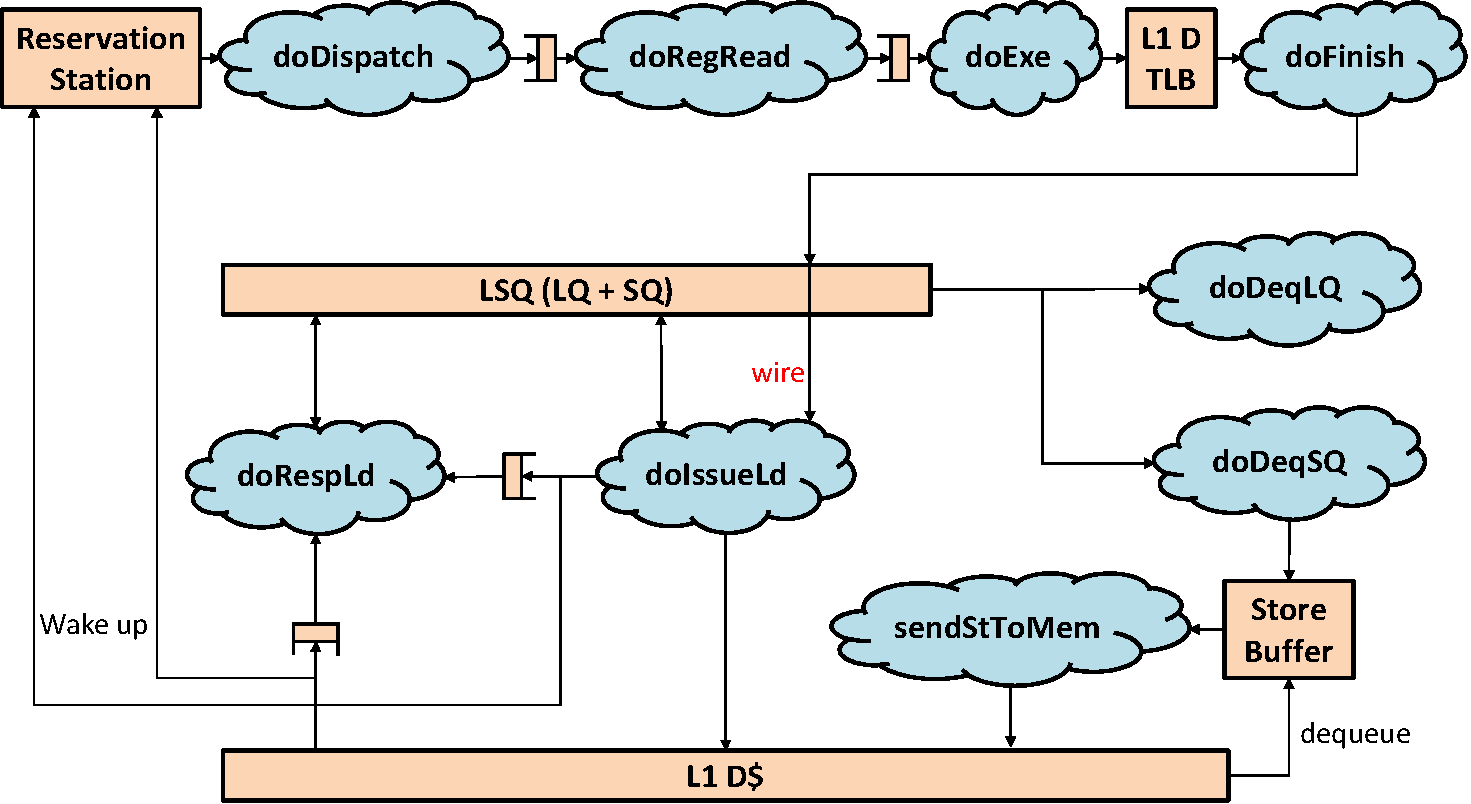
\includegraphics[width=\columnwidth]{fig/mem_exe_crop.pdf}
    \caption{Implementation of the memory execution pipeline}\label{fig:mem-exe-pipe-impl}
\end{figure}

Figure~\ref{fig:mem-exe-pipe-impl} shows the implementation of the memory execution pipeline.
It contains the following internal rules:
\begin{itemize}
    \item Rule \code{doDispatch}: retrieves a ready instruction from the reservation station.
    \item Rule \code{doRegRead}: reads the source-register values.
    This rule also checks for data bypassing from the ALU execution pipelines.
    \item Rule \code{doExe}: calculates the virtual address, sends to D TLB, and computes store data if applicable.
    \item Rule \code{doFinish}: gets the translation results, updates ROB entry, and updates the LSQ entry.
    If the instructions is a normal load without page faults, then the load address is recorded in a \emph{wire}, and the \code{doIssueLd} rule may use this wire to issue this load to memory immediately in the same cycle.
    \item Rule \code{doIssueLd}: issues a load to execution, i.e., first search LSQ and store buffer for forwarding.
    If forwarding is available, then The forwarding result will be enqueued to a FIFO which will be dequeued by the \code{doRespLd} rule, and we wake up dependent instructions in the reservation stations and update the aggressive scoreboard.
    Otherwise, we request memory.
    The \code{doIssueLd} rule can get the ready-to-issue load from the wire set by the \code{doFinish} rule, or from the \code{getIssueLd} method of LSQ.
    We give priority to the wire.
    \item Rule \code{doRespLd}: get load responses from either the FIFO containing forwarding results or the L1 D cache.
    It updates the LSQ entry, conservative scoreboard and physical register file.
    The aggressive scoreboard and reservation stations are updated in earlier cycles when the forwarding result or cache data is available.
    \item Rule \code{doDeqLQ}: dequeues the LQ.
    In case the dequeued entry is a load-reserve or MMIO access, we need to first execute it.
    (The execution requires a new rule which is not shown here.)
    \item Rule \code{doDeqSQ}: dequeues the SQ.
    In case the dequeued entry is a load-reserve or MMIO access, we need to first execute it.
    (The execution requires a new rule which is not shown here.)
    If the dequeued entry is a normal store, then we put it into the store buffer in case of WMM.
    In case of TSO (which is not shown in the figure), we need to first execute the store in the memory system.
    \item Rule \code{sendStToMem}: retrieves a read-to-issue store address from the store buffer and requests L1 D cache.
    When the store completes in the D cache, D cache will call the \code{deq} method of store buffer to remove the entry.
\end{itemize}

\subsubsection{Source Code}
See module \code{mkMemExePipeline} in \code{//procs/RV64G\_OOO/MemExePipeline.bsv}.
